A digital image is a two-dimensional discrete function $I(x, y)$ defined over a finite grid of integer coordinates. Each ordered pair $(x, y)$ refers to a spatial location in the image plane, and the corresponding value $I(x, y)$ denotes the intensity — or brightness — measured at that position. In standard grayscale images, the intensity values range over a finite interval, typically $[0, 255]$, where $0$ represents black and $255$ represents white. Intermediate values encode proportional levels of gray.

This allows images to be treated as matrices of numerical data. Each row corresponds to a horizontal slice through the image, and each column to a vertical slice. The array format aligns with standard data structures in numerical computing, enabling efficient storage, manipulation, and analysis using linear algebraic tools. More importantly, this view enables the application of discrete transformations that operate directly on the pixel grid.

The array-based nature of digital images reflects their method of acquisition. Optical sensors — such as charge-coupled devices (CCDs) — sample incoming light intensity across a regular lattice of photodetectors. Each photodetector integrates the radiance over a small rectangular region and records the result as a scalar value. This process discretizes a continuous visual field, replacing smooth spatial variation with a piecewise-constant approximation.

Despite this discretization, many natural images exhibit local continuity. In regions of uniform texture or lighting, adjacent pixels tend to have similar intensity values. This results in spatial smoothness — a statistical tendency that can be exploited by various image processing algorithms. Conversely, abrupt changes in intensity may indicate the presence of physical boundaries, surface discontinuities, or occlusion contours.

The goal of low-level image processing is to extract global geometric elements from the raw intensity field — to identify where transitions occur, how they are oriented, and how they combine to form recognizable configurations. The first step in this process is edge detection: identifying where intensity values change significantly in space.

To extract localized transitions in brightness, digital image processing employs gradient-based methods. These techniques compute spatial derivatives of the intensity function $I(x, y)$ using discrete convolution kernels. Common approximations include the Sobel, Prewitt, or central difference operators, which estimate the partial derivatives $\partial I / \partial x$ and $\partial I / \partial y$ by combining intensities in a small neighborhood.

The result of this process is a vector field $G(x, y) = (I_x(x, y), I_y(x, y))$, where $I_x$ and $I_y$ denote the horizontal and vertical gradients respectively. The magnitude of this vector, defined as
\[
\|G(x, y)\| = \sqrt{I_x(x, y)^2 + I_y(x, y)^2},
\]
quantifies the rate of change in brightness at each pixel. The direction $\theta(x, y) = \arctan2(I_y, I_x)$ indicates the orientation of maximal contrast — that is, the direction perpendicular to the local edge.

To reduce the resulting field to a usable form, a fixed threshold is applied to the gradient magnitude. The binary edge map $E(x, y)$ is defined by
\[
E(x, y) =
\begin{cases}
1 & \text{if } \|G(x, y)\| > \tau, \\
0 & \text{otherwise},
\end{cases}
\]
where $\tau$ is a positive scalar threshold. The outcome is a sparse array in which $E(x, y) = 1$ denotes an edge candidate and $0$ otherwise. This thresholding step suppresses minor fluctuations while preserving strong transitions, isolating regions of significant spatial variation.

The resulting edge map retains only local information. Each nonzero pixel marks a point of abrupt contrast but encodes no higher-order structure. It does not indicate whether a given edge continues across neighboring pixels, nor whether multiple edge points are aligned.

In many visual tasks, the detection of straight lines is the second step after edge detection. Lines may correspond to physical edges in man-made environments — such as walls, roads, or tools — or to object boundaries under specific perspectives. In medical imaging, remote sensing, and industrial inspection, linear features often identify critical diagnostic or structural information.

However a straight line is not a local construct. Unlike a gradient, which depends only on immediate neighbors, a line is a global configuration — a set of pixels that, despite spatial separation, conform to a shared geometric constraint. In the discrete setting, this constraint must be inferred from partial and often noisy evidence. The edge map contains a large number of isolated pixels, many of which are spurious. Determining which subsets form lines requires aggregating across potentially distant points.

One naïve approach is to enumerate all pairs of edge pixels and test whether a third or fourth point lies along the same line. Given $n$ detected edge points, there are $\binom{n}{2}$ possible pairs, and each pair defines a candidate line. For each such line, one must then check whether additional points fall sufficiently close to it, accounting for quantization and discretization artifacts. The combinatorial burden of this process grows quadratically in the number of edge pixels and becomes intractable at practical image resolutions.

The challenge is further exacerbated by noise and occlusion. Genuine lines may be broken into disconnected segments, and false positives may arise from texture or illumination variations. Any method that seeks to identify lines must accommodate partial evidence and operate under pixel-level uncertainty. The core problem is not to test a single hypothesis, but to efficiently search a vast and noisy hypothesis space for a small number of consistent patterns.
To detect lines in a binary edge map, one may adopt a parametric formulation of straight lines. In Cartesian coordinates, the general equation for a line is $y = mx + b$, where $m$ is the slope and $b$ the vertical intercept. The goal is to identify parameter pairs $(m, b)$ that describe lines passing through multiple edge pixels.

Each edge pixel $(x_0, y_0)$ imposes a constraint on the set of valid $(m, b)$ values. Specifically, if a line passes through $(x_0, y_0)$, then its parameters must satisfy
\[
y_0 = m x_0 + b,
\quad \text{or equivalently,} \quad
b = y_0 - m x_0.
\]
This relation defines a one-dimensional locus in the $(m, b)$ parameter space: the set of all lines that intersect $(x_0, y_0)$. For fixed $x_0$ and $y_0$, this is a straight line in parameter space — each pixel generates such a line of possible $(m, b)$ values.

To implement this idea computationally, the $(m, b)$ space is discretized into a finite grid. A two-dimensional accumulator array is initialized, with each cell corresponding to a quantized pair of slope and intercept values. For each edge pixel, the algorithm evaluates the above relation at discrete samples of $m$ and computes the corresponding $b$ values. Each resulting $(m_i, b_i)$ pair increments the count in its associated cell of the accumulator.

After processing all edge pixels, the accumulator stores the number of pixels consistent with each candidate line. Peaks in this array — cells with significantly elevated counts — represent line parameters that are supported by many pixels. These peaks are interpreted as strong linear features in the original image.

While this method organizes the problem effectively, it remains computationally intensive. Each edge pixel must evaluate the constraint over all discretized slope values, resulting in a cost proportional to the product of the number of edge pixels and the number of slope samples. Moreover, the parameterization becomes unstable for nearly vertical lines, where $m$ diverges. These limitations motivate the adoption of alternative representations, but the core insight remains: transform each pixel into a family of candidate lines, and identify agreement via intersection in parameter space.

The Hough transform discretizes the $(m, b)$ space into a finite grid. For each edge pixel, it iterates over a predefined set of slope values $m_i$ and computes $b_i = y - m_i x$. A two-dimensional accumulator array stores how many pixels vote for each parameter pair $(m_i, b_i)$. After all edge pixels have contributed, cells in the accumulator with high vote counts correspond to lines that are strongly supported by the data.

This formulation avoids the combinatorial explosion of testing all pixel pairs. Each pixel acts independently, voting for a family of possible lines. Lines with high support appear as peaks in the accumulator, which can be located efficiently using standard search techniques.

In practice, this classical parameterization has limitations near vertical lines, where the slope $m$ becomes unbounded. A more robust formulation employs the normal parameterization $\rho = x\cos\theta + y\sin\theta$, which describes lines using distance and orientation. This variant ensures uniform treatment of all orientations, but the essential idea remains: transform alignment in image space into intersection in parameter space, and use voting to identify consistent structures.

The strength of the Hough transform lies in its ability to transform the problem from image space to parameter space. Once the core mechanism is established — each edge pixel voting for the set of parameters consistent with its location — the method generalizes seamlessly to more complex shapes.

For example, consider the problem of detecting circles. A circle in the plane is defined by the equation
\[
(x - a)^2 + (y - b)^2 = r^2,
\]
where $(a, b)$ denotes the center and $r$ the radius. Each edge pixel $(x_0, y_0)$ must satisfy this relation for some triplet $(a, b, r)$. If the radius is fixed, then every such pixel defines a circular locus of possible centers — that is, it contributes votes to all $(a, b)$ such that $(x_0 - a)^2 + (y_0 - b)^2 = r^2$. Allowing $r$ to vary introduces a third dimension: the accumulator now becomes a 3D volume over $(a, b, r)$.

This generalizes further. Any shape that admits an algebraic parameterization can be detected in the same way. For instance:

\begin{itemize}
  \item \textbf{Ellipses} require five parameters: center coordinates, major and minor axis lengths, and orientation.
  \item \textbf{Parabolas} can be parameterized by vertex location and opening direction.
  \item \textbf{Arbitrary curves} described by parametric equations or algebraic forms can be handled, provided the number of parameters is finite and reasonably small.
\end{itemize}

In each case, the edge pixel votes for a hypersurface in the corresponding parameter space. The transform aggregates these votes, and high-density regions in the accumulator indicate the presence of shapes that are strongly supported by the edge data.

The cost of generality is dimensional: for a shape defined by $k$ parameters, the accumulator array lives in $\mathbb{R}^k$. Memory and computation scale exponentially with $k$, limiting the practical complexity of detectable shapes. Nevertheless, for many applications — especially where the shape class is known and low-dimensional — the Hough transform remains a tractable and robust detection mechanism.

\vspace{50em}

\begin{figure}[ht]
  \centering
  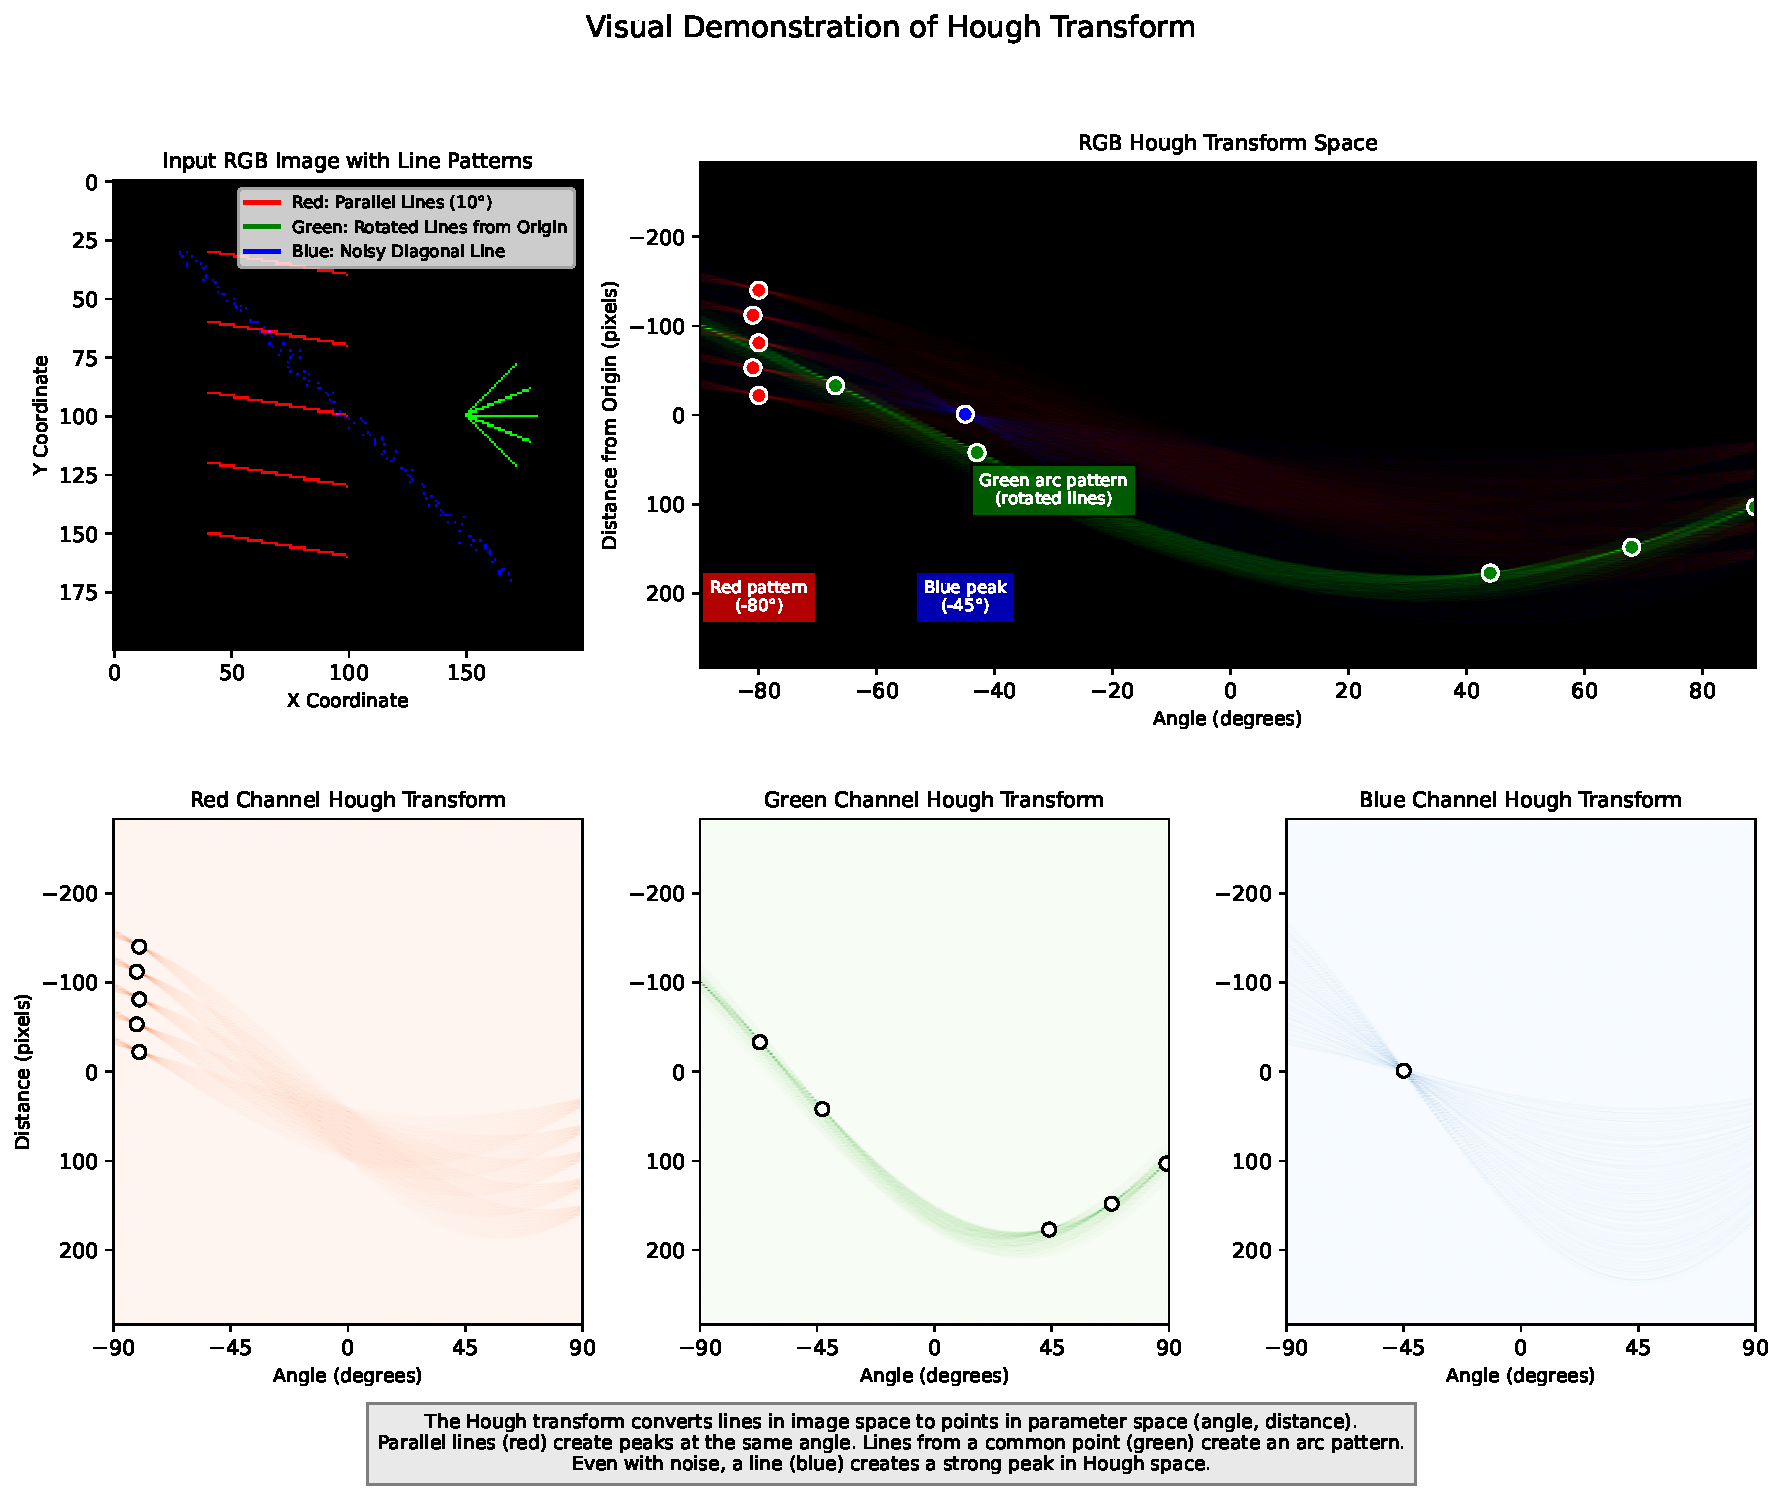
\includegraphics[width=1\textwidth]{41_HoughTransfrom/hough_transform_visualization.pdf}
  \label{fig:permgraph3}
\end{figure}
